\section{Theoretical Analysis}
\label{sec:analysis}

In this section, the circuit shown in Figure~\ref{fig:t1draw} is analysed
theoretically, in terms of its time and frequency responses.

\section{Time response}

The circuit consists of a single V-R-C loop where a current $i(t)$ circulates. The
voltage source $v_I(t)$ drives its input, and the output voltage $v_O(t)$ is taken from
the capacitor terminals. Applying the Kirchhoff Voltage Law (KVL), a single
equation for the single loop in the circuit can be written as




\begin{figure}[h] \centering
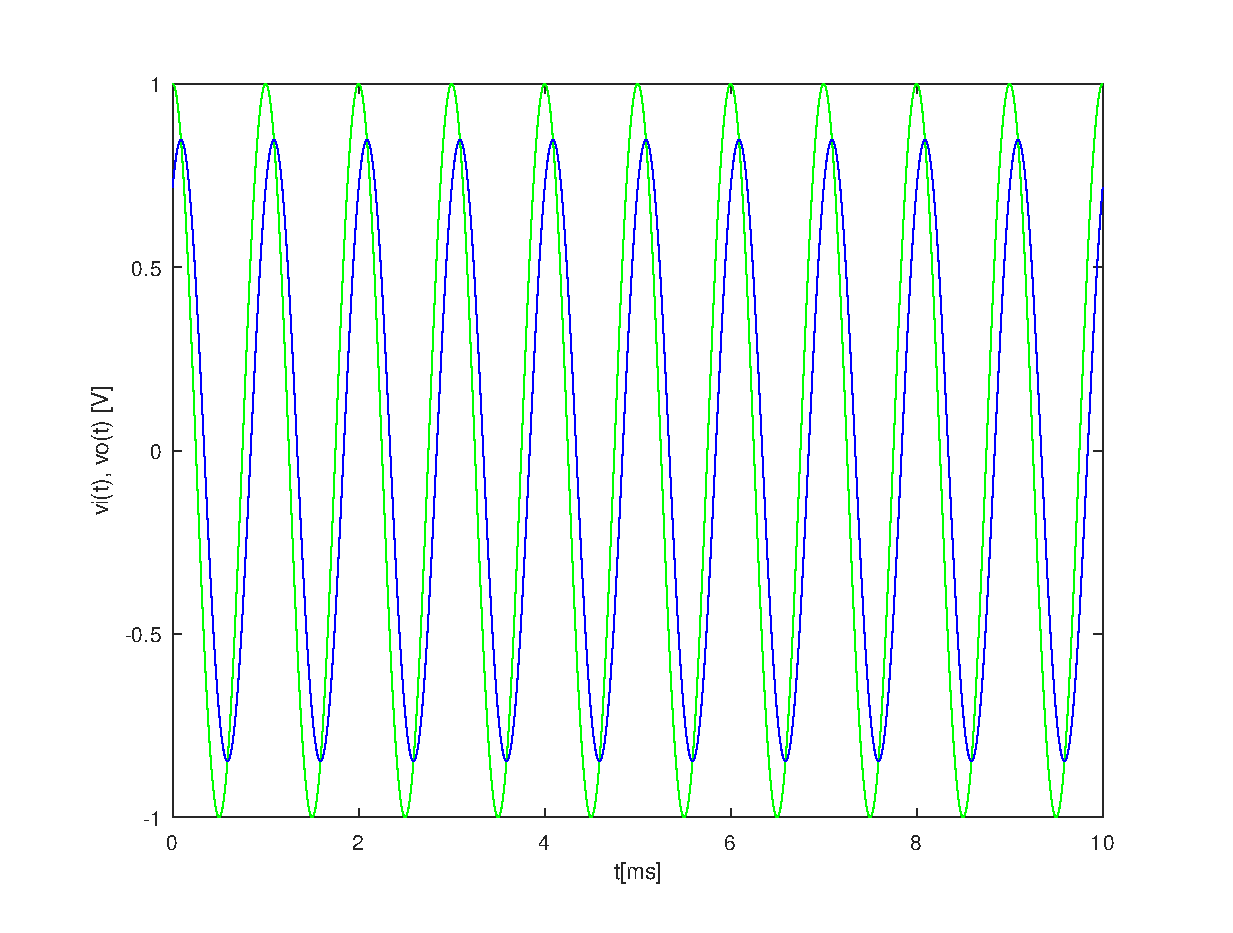
\includegraphics[width=0.8\linewidth]{forced.eps}
\caption{Forced sinusoidal response.}
\label{fig:forced}
\end{figure}

\section{Frequency response}

\lipsum[1-1]


